\documentclass[10pt]{article}
\usepackage[T1]{fontenc}
\usepackage{amsmath}
\usepackage{tikz}
\usetikzlibrary{arrows.meta}
\pagestyle{empty}
% Compile with pdflatex. The page is cropped to the vector artwork.
\newsavebox{\mapbox}
\begin{document}
\begin{lrbox}{\mapbox}
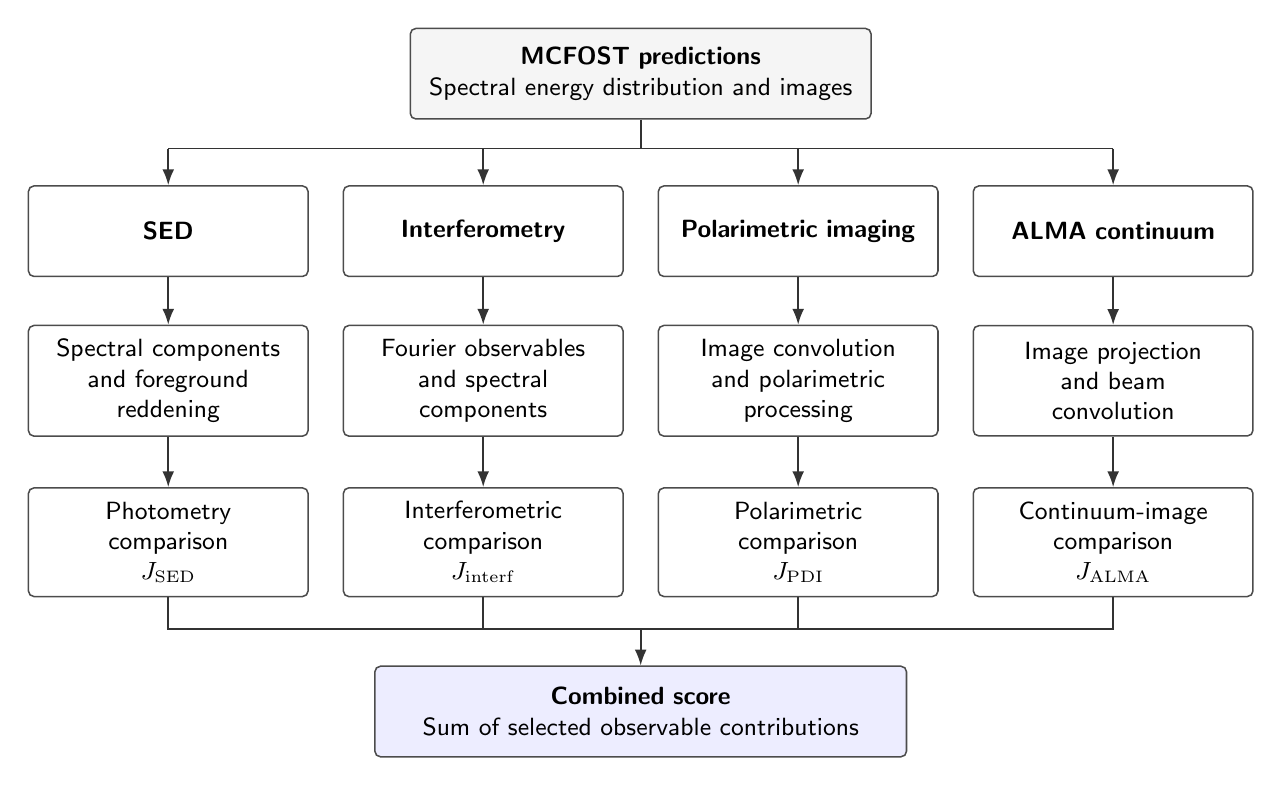
\begin{tikzpicture}[
  box/.style={draw=black!70,line width=0.55pt,rounded corners=2pt,
    align=center,font=\sffamily\small,inner sep=5pt,minimum height=1.15cm},
  inputbox/.style={box,fill=black!4},
  searchbox/.style={box,fill=blue!7},
  arrow/.style={-{Latex[length=2mm]},line width=0.65pt,draw=black!80},
  wire/.style={line width=0.65pt,draw=black!80}
]

\node[inputbox,text width=5.5cm] (predictions) at (6,2)
  {\textbf{MCFOST predictions}\\Spectral energy distribution and images};
\node[box,text width=3.2cm] (sed) at (0,0)
  {\textbf{SED}};
\node[box,text width=3.2cm] (interf) at (4,0)
  {\textbf{Interferometry}};
\node[box,text width=3.2cm] (pdi) at (8,0)
  {\textbf{Polarimetric imaging}};
\node[box,text width=3.2cm] (alma) at (12,0)
  {\textbf{ALMA continuum}};
\node[box,text width=3.2cm,minimum height=1.4cm] (sedproc) at (0,-1.9)
  {Spectral components\\and foreground\\reddening};
\node[box,text width=3.2cm,minimum height=1.4cm] (intproc) at (4,-1.9)
  {Fourier observables\\and spectral\\components};
\node[box,text width=3.2cm,minimum height=1.4cm] (pdiproc) at (8,-1.9)
  {Image convolution\\and polarimetric\\processing};
\node[box,text width=3.2cm,minimum height=1.4cm] (almaproc) at (12,-1.9)
  {Image projection\\and beam\\convolution};
\node[box,text width=3.2cm,minimum height=1.35cm] (sedcost) at (0,-3.95)
  {Photometry\\comparison\\$J_{\rm SED}$};
\node[box,text width=3.2cm,minimum height=1.35cm] (intcost) at (4,-3.95)
  {Interferometric\\comparison\\$J_{\rm interf}$};
\node[box,text width=3.2cm,minimum height=1.35cm] (pdicost) at (8,-3.95)
  {Polarimetric\\comparison\\$J_{\rm PDI}$};
\node[box,text width=3.2cm,minimum height=1.35cm] (almacost) at (12,-3.95)
  {Continuum-image\\comparison\\$J_{\rm ALMA}$};
\node[searchbox,text width=6.4cm] (total) at (6,-6.1)
  {\textbf{Combined score}\\Sum of selected observable contributions};
\draw[wire] (predictions.south) -- (6,1.05);
\draw[wire] (0,1.05) -- (12,1.05);
\foreach \n in {sed,interf,pdi,alma}
  \draw[arrow] (\n.north |- 0,1.05) -- (\n.north);
\draw[arrow] (sed) -- (sedproc);
\draw[arrow] (interf) -- (intproc);
\draw[arrow] (pdi) -- (pdiproc);
\draw[arrow] (alma) -- (almaproc);
\draw[arrow] (sedproc) -- (sedcost);
\draw[arrow] (intproc) -- (intcost);
\draw[arrow] (pdiproc) -- (pdicost);
\draw[arrow] (almaproc) -- (almacost);
\draw[wire] (sedcost.south) -- (0,-5.05) -- (12,-5.05) -- (almacost.south);
\draw[wire] (intcost.south) -- (4,-5.05);
\draw[wire] (pdicost.south) -- (8,-5.05);
\draw[arrow] (6,-5.05) -- (total.north);

\end{tikzpicture}
\end{lrbox}
\pdfpagewidth=\dimexpr\wd\mapbox+12pt\relax
\pdfpageheight=\dimexpr\ht\mapbox+\dp\mapbox+12pt\relax
\pdfhorigin=0pt
\pdfvorigin=0pt
\shipout\vbox{\offinterlineskip\kern6pt\hbox{\kern6pt\usebox{\mapbox}\kern6pt}\kern6pt}
\end{document}
